\documentclass[conference]{IEEEtran}
\IEEEoverridecommandlockouts
\usepackage{cite}
\usepackage{amsmath,amssymb,amsfonts}
\usepackage{algorithmic}
\usepackage{graphicx}
\usepackage{textcomp}
\usepackage[euler]{textgreek}
\usepackage{xcolor}
\usepackage[utf8]{inputenc}
\usepackage[T1]{fontenc}
\usepackage[english]{babel}
\usepackage{hyphenat}
\usepackage{indentfirst}
\usepackage{graphicx}
\usepackage{verbatim}
\usepackage{listings}
\usepackage{url}
\usepackage{stringenc}
\usepackage{pdfescape}
\usepackage{subfig}
\usepackage{float}
\usepackage{eurosym}
\usepackage[toc,page]{appendix}
\usepackage{longtable}
\usepackage{graphicx}
\usepackage[export]{adjustbox}
\graphicspath{ {images/} }
\usepackage{listings}
\usepackage{makecell}
\usepackage{float}
\usepackage{enumitem}
\usepackage[table]{xcolor}
\usepackage{booktabs}
\usepackage{multirow}
\usepackage[color]{vdmlisting}
\usepackage{listings}
\usepackage[hidelinks]{hyperref}
\usepackage{todonotes}
\def\BibTeX{{\rm B\kern-.05em{\sc i\kern-.025em b}\kern-.08em
    T\kern-.1667em\lower.7ex\hbox{E}\kern-.125emX}}
\begin{document}

\title{Line Following and Obstacle Avoidance behaviours for AlphaBot2 RPi - real and simulated}

\author{\IEEEauthorblockN{Diogo Serra Duque}
\IEEEauthorblockA{\textit{Faculdade de Engenharia da Universidade do Porto} \\
Rua Dr. Roberto Frias \\
4200-465 Porto, Portugal \\
up201406274@fe.up.pt}
\and
\IEEEauthorblockN{Sara Filipa Couto Fernandes}
\IEEEauthorblockA{\textit{Faculdade de Engenharia da Universidade do Porto} \\
Rua Dr. Roberto Frias \\
4200-465 Porto, Portugal \\
up201405955@fe.up.pt}
}

\maketitle

\begin{abstract}
Nowadays, more and more autonomous robots are used, with the ability to follow a certain line or, specially, to detect obstacles, like the typical behaviour of a human being, for example. Thus, this article presents the implementation of an algorithm that allows to move an autonomous robot, Alphabot2 RPi, either real or simulated through Gazebo, and the execution of both simultaneously. These robots use upper and lower sensors to detect obstacles and lines, making it a reactive robot capable of responding to a world of which it has no previous knowledge. To verify that the implementation is executed in the same way by the real and simulated robot, the error between the times each robot takes to go through the tracks created. By analyzing these results, it was verified that there are discrepancies between the values of the real robot and the simulated robot, maybe because the simulated robot is not modeled exactly like the real Alphabot2 RPi, and there may be errors in its dimensions, causing problems in its execution.
\end{abstract}

\begin{IEEEkeywords}
robot, AlphaBot2 RPi, simulation, ROS, line following, obstacle avoidance
\end{IEEEkeywords}

\section{Introduction} \label{intro}

The AlphaBot2 RPi is a small robot, composed by 5 lower ITR20001/T, reflective infrared photoelectric sensors, for line tracking and 2 superior ST188, reflective infrared photoelectric sensors, for obstacle avoiding. This robot uses a Raspberry Pi 3 which is a small computer with the Raspbian operating system, so that it is possible to move the respective robot. Alphabot also has a Raspberry Pi camera which can be used for various purposes\footnote{\url{https://www.waveshare.com/wiki/AlphaBot2}}.

The present experimental activity focuses on implementing the different sensors of the AlphaBot2 RPi in the real robot as well as in the simulated robot, through Gazebo which is a robot and world simulator\footnote{\url{http://gazebosim.org}} and ROS (Robot Operating System)\footnote{\url{http://www.ros.org}}. The 5 lower sensors are intended to detect lines, allowing the robot to follow them, while the 2 upper sensors aim to detect obstacles. All the simulations were created using the Gazebo and its plugins, namely the laser sensor or camera sensor plugins as well as ROS commands. As for the real robot, it implements commands related to the Raspberry Pi that allow the programming of the AlphaBot hardware. Also, a track similar to the track used in the Conde project\cite{b1, b2, b3} was used, with smaller dimensions, for test purposes.

As regards the division of this article, it can be seen that it is divided into 5 main sections, including this section (Section \ref{intro}). Section \ref{relwork} presents the state of the art or projects related to the main purpose of this activity. Section \ref{alpha} refers to the AlphaBot2 RPi robot used, including the main objectives of this experiment (Subsection \ref{goal}), as well as the robot specification (Section \ref{spec}), containing the real (Subsection \ref{spec_real}) and simulated robot specs (Subsection \ref{spec_sim}). Also in Section \ref{alpha}, the behaviour of the robot (Subsection \ref{behaviour}), the world or environment in which the robot is tested (Subsection \ref{world}), the Alphabot2 RPi architecture used (Subsection \ref{ros}), as well as the approach implemented (Subsection \ref{alg}), are presented so that the robot could follow lines and avoid obstacles. Finally, we have the analysis of the results obtained, in Section \ref{results} and the conclusions drawn from this activity, in Section \ref{conclusions}.

\section{Related Work} \label{relwork}

These days, the area of robotics is increasingly being explored, and for this reason there are a huge number of studies, experimental activities and works related to line following and obstacle avoidance robots.

In \cite{b4}, it is presented a robot that achieves high speeds and at the same time follows lines independently, combining both human experience and experimental data extracted from a trained neural network. This robot uses the novel square-topology infrared sensor matrix that allows you to anticipate a turn by sensing a curve ahead.

In \cite{b5}, image preprocessing is used for line following robots, through the Track-Before-Detect algorithm that uses the Viterbi algorithm. In addition, this robot and its algorithms use deep learning to estimate the line and the area beyond the line.

The robot presented in \cite{b6} is one with multiple destinations and with multiple lines to follow, where the line that the robot must follow comes from user inputs. This robot is smart enough to avoid collisions with obstacles as it travels its path, returning to its initial position when it finishes its course.

The article \cite{b7} presents an algorithm that allows a wheeled robot to follow a path and to avoid obstacles that cross in front of him.

The article \cite{b8} proposes an algorithm that uses Cartesian-to-polar conversion tracklets with the Viterbi algorithm to estimate the line to be followed. Since the line may have a reduced contrast, Monte Carlo tests are used to analyze the properties of the main algorithm used.

The robot presented in \cite{b9} is a fuzzy obstacle avoidance system for an elderly-assistant and walking-assistant robot (EWR) using two ultrasonic sensors that exist on the front of the robot.

Finally, paper \cite{b10} describes the implementation of a method that efficiently detects and avoids obstacles through a 2D LiDAR of an autonomous robot. This method extracts spatial information from a point-cloud laser using segmentation and clustering methods. In order to detect the geometric structure of the obstacle, the Convex hull algorithm was used.

Despite these advances, there is no robot that follows lines and detect obstacles at the same time that a simulation tries to fulfill these same tasks and objectives.

\section{AlphaBot2 RPi Simulation} \label{alpha}

\subsection{Main Goal} \label{goal}

This activity has 3 distinct goals. The first one is about getting the AlphaBot2 RPi, either real or simulated, to be able to follow lines. The second is similar to the first, only this time the robot has to be able to detect and avoid obstacles. The third objective is related to the synchronization of the real and simulated robot, allowing them to be executed and tested at the same time.

These objectives and tasks are further complemented by the work developed by \cite{b1, b2, b3}, where the camera of the Conde robot is programmed to make the robot able to stop when it sees an obstacle or a treadmill, respecting the traffic signals.

\subsection{Robot Specification} \label{spec}

In this section, the real AlphaBot2 RPi and the one simulated on Gazebo will be specified.

\subsubsection{Real Robot Specification} \label{spec_real}

The Alphabot2 RPi robot consists of the robot chassis and an AlphaBot2-Pi adapter board to support a Raspberry Pi.

Due to its highly modular design, this robot can be mounted without too much effort or additional tools.

There are different accessories that can be used by this robot, however in this article will be presented an Alphabot2 with its basic components.

Figure \ref{fig:fig1} shows the fully assembled robot with its basic components.

\begin{figure}[H]
    \centering
    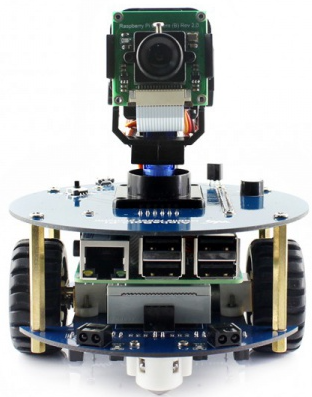
\includegraphics[width=2.7cm]{Alphabot2.png}
    \caption{AlphaBot2 RPi assembled}
    \label{fig:fig1}
\end{figure}

The bottom board, which serves as the base of the robot, has different components that must be identified (Figure \ref{fig:fig2}).

\begin{figure}[H]
    \centering
    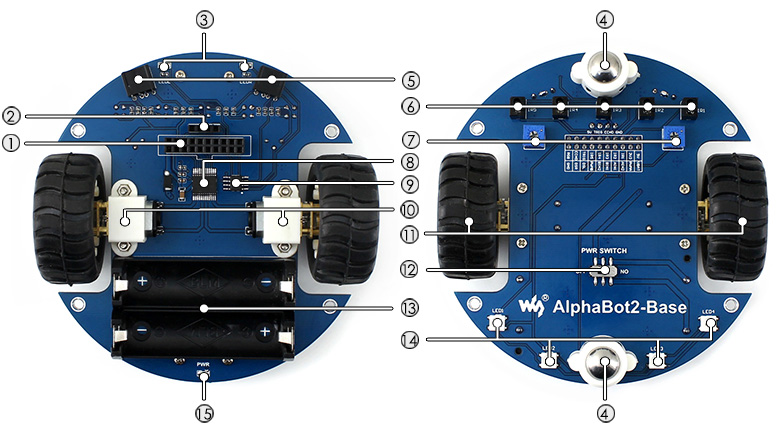
\includegraphics[width=9.50cm]{AlphaBot2-Base-intro.jpg}
    \caption{AlphaBot2 RPi base board}
    \label{fig:fig2}
\end{figure}

This board consists of the following components:

\begin{enumerate}
    \item Ultrasonic module interface
    \item AlphaBot2 control interface: for connecting sorts of controller adapter board
    \item Obstacle avoiding indicators
    \item Omni-direction wheel
    \item ST188: reflective infrared photoelectric sensor, for obstacle avoiding
    \item ITR20001/T: reflective infrared photoelectric sensor, for line tracking
    \item Potentiometer for adjusting obstacle avoiding range
    \item TB6612FNG dual H-bridge motor driver
    \item LM393 voltage comparator
    \item N20 micro gear motor reduction rate 1:30, 6V/600RPM
    \item Rubber wheels diameter 42mm, width 19mm
    \item Power switch
    \item Battery holder: supports 14500 batteries
    \item WS2812B: true color RGB LEDs
    \item Power indicator
\end{enumerate}

The connection to Raspberry Pi is made through the top board (Figure \ref{fig:fig3}).

\begin{figure}[H]
    \centering
    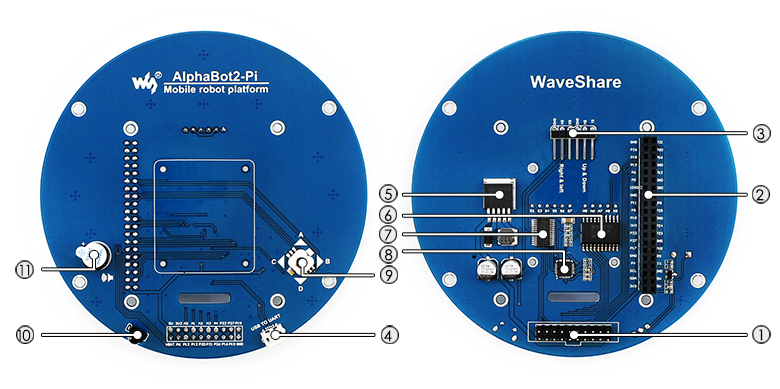
\includegraphics[width=9.50cm]{AlphaBot2-Pi-intro.jpg}
    \caption{AlphaBot2 RPi connection to Raspberry Pi}
    \label{fig:fig3}
\end{figure}

This board has the following components:

\begin{enumerate}
    \item AlphaBot2 control interface: for connecting AlphaBot2-Base
    \item Raspberry Pi interface: for connecting Raspberry Pi 3 Model B
    \item Servo interface
    \item USB TO UART: easy for controlling the Pi via UART
    \item LM2596: 5V voltage regulator
    \item TLC1543: 10-bit AD acquisition chip, allows the Pi to use analog sensors
    \item PCA9685: servo controller, make it more smoothly to rotate the pan head
    \item CP2102: USB TO UART converter
    \item Joystick
    \item IR receiver
    \item Buzzer
\end{enumerate}

\subsubsection{Simulated Robot Specification} \label{spec_sim}

For the construction of the simulated robot, we tried to use the real dimensions of the Alphabot2 RPi.

Since many robot components did not need to be simulated, only a robot with the chassis, sensors, wheels, casters and camera was created, where the positions of these components are the same as the positions they occupy in the real robot.

The whole simulated robot was implemented using a .xacro file that is executed in the Gazebo, in which only the chassis and the camera are represented through meshes and the remaining forms through simple geometries.

Thus, this simulated robot will have 5 lower sensors, with a vertical scan to detect lines and 2 upper sensors with a range between -15 degrees and 15 degrees, making a total of 30 degrees and a minimum distance of 1cm and maximum of 10cm. For line detection sensors, it was used the Gazebo plugin for a camera type sensor and for the obstacle detection was used the plugin that creates laser sensors.

The final look of the simulated robot can be visualized in Figure \ref{fig:fig4}.

\begin{figure}[H]
    \centering
    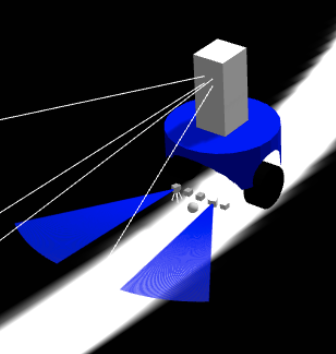
\includegraphics[width=6cm]{Simulated-robot.png}
    \caption{AlphaBot2 RPi simulated on Gazebo}
    \label{fig:fig4}
\end{figure}

\subsection{Robot Behaviour} \label{behaviour}

This robot follows a subsumption based architecture as the one shown in Figure \ref{fig:fig5}.

\begin{figure}[H]
    \centering
    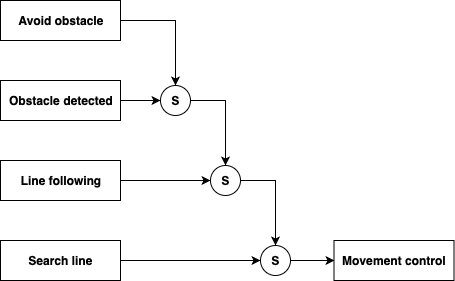
\includegraphics[width=8.5cm]{Subsumption.png}
    \caption{Subsumption based architecture}
    \label{fig:fig5}
\end{figure}

According to the architecture, the robot presents only 4 possible behaviours, being the first representative of the initial movement, the second one relative to the line following, the third related to obstacles detection and the fourth and last one related to the obstacles avoidance.

Initially, the robot moves itself around the map searching for a line (initial movement). As soon as the robot detects a line, it follows the respective line. 

Then, if the robot's sensors detect an obstacle it will assume another behaviour, in order to avoid the collision of the robot with that obstacle.

If the obstacle is to the left of the robot, it has to deviate from the right and vice versa. If the obstacle is in front of the robot it can deviate from either the left or the right.

\subsection{World} \label{world}

Initially, the world/track created for the simulated robot to be tested was an adaptation of the track used by Conde\cite{b1, b2, b3}.

Conde's track is an extensive track, with two carriage ways, a treadmill and traffic lights that indicated whether or not the robot could move forward. In addition, this lane could have some obstacles in its way, which the robot would have to avoid. Figure \ref{fig:fig6} represents the Conde's world.

\begin{figure}[H]
    \centering
    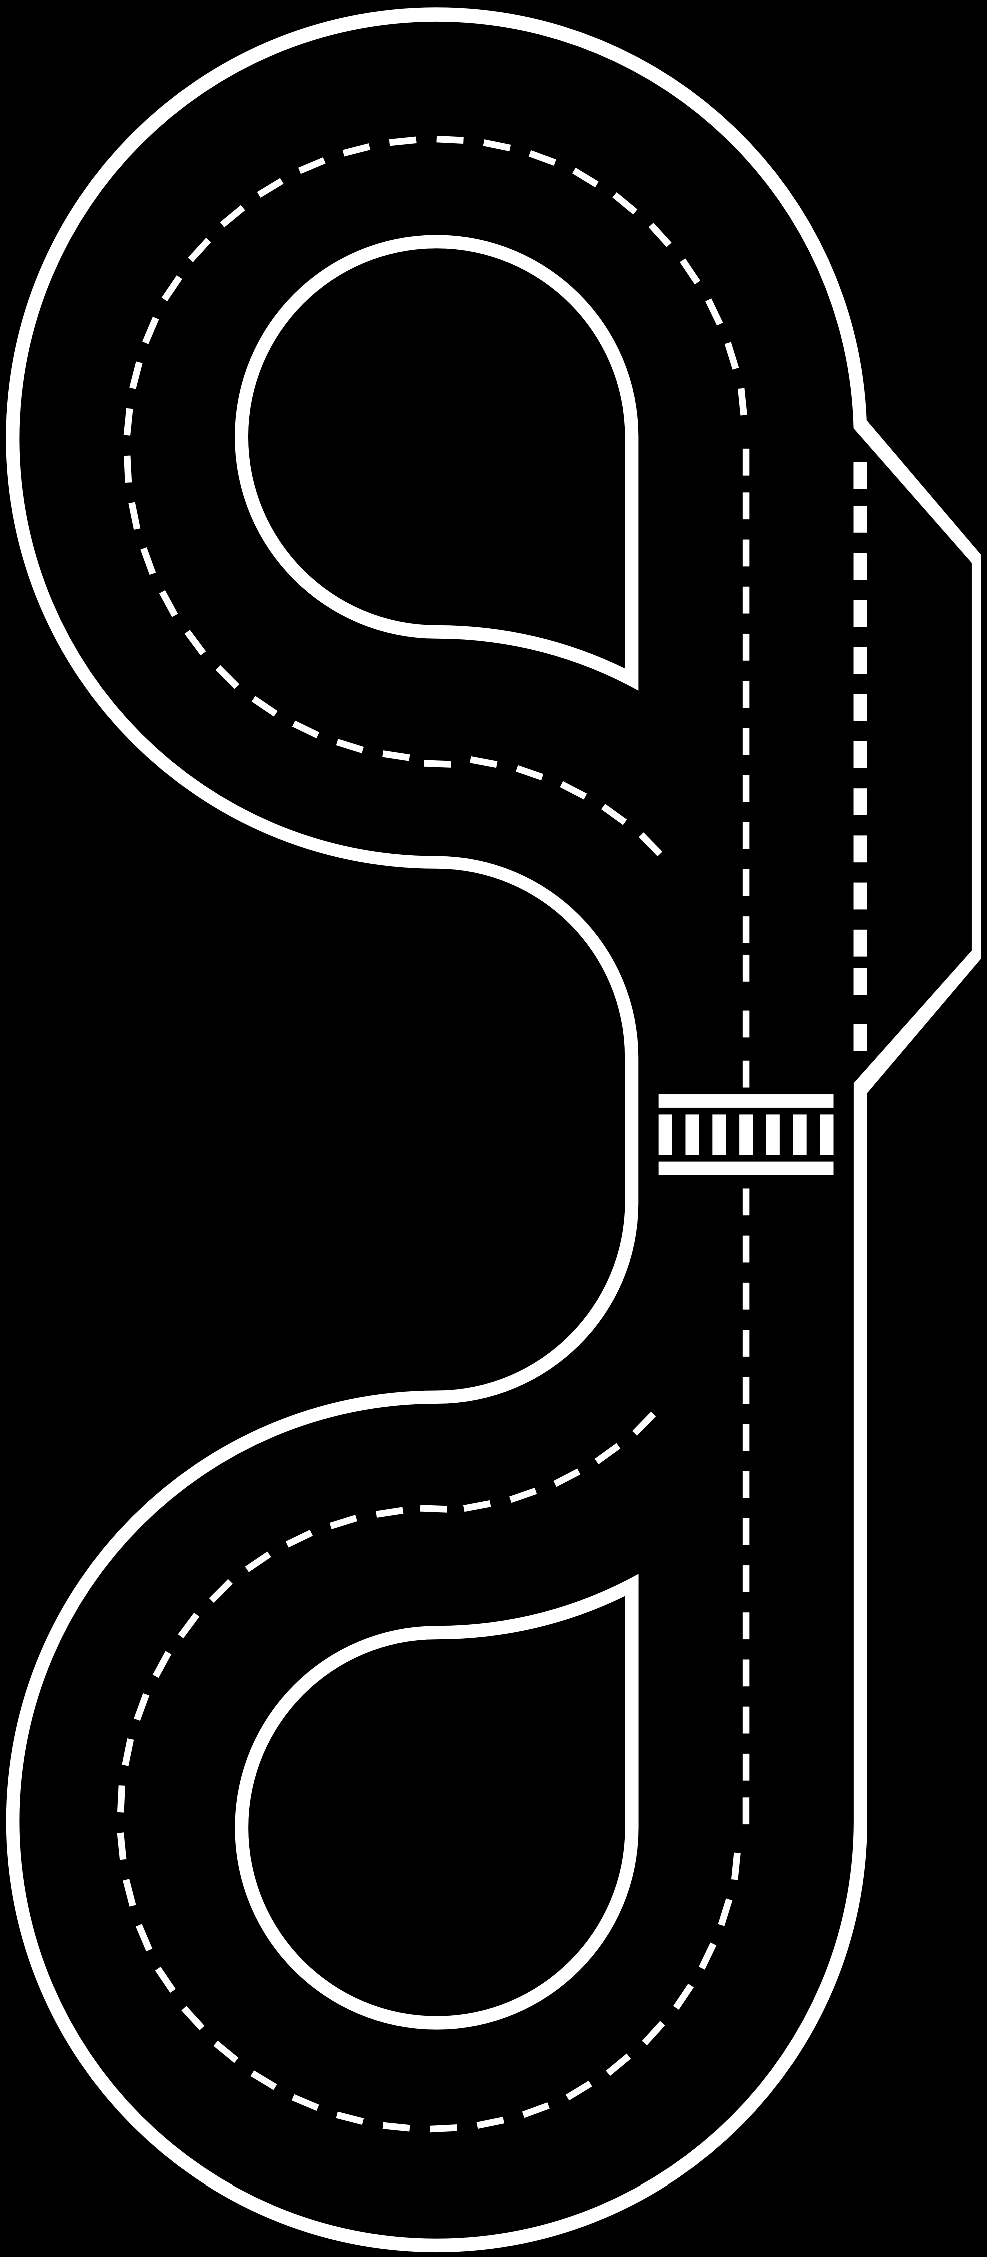
\includegraphics[width=2cm]{Conde-track.png}
    \caption{Conde's world}
    \label{fig:fig6}
\end{figure}

The track created for the AlphaBot2 RPi is therefore an adaptation of the Conde's world. Figure \ref{fig:fig7} shows the track adapted for the AlphaBot2 RPi.

\begin{figure}[H]
    \centering
    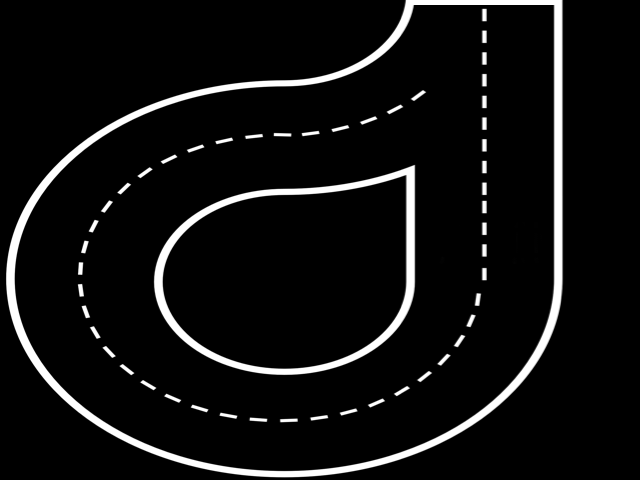
\includegraphics[width=3cm]{AB2-track.png}
    \caption{Alphabot2 RPi's world}
    \label{fig:fig7}
\end{figure}

Although this new track was created, two simpler tracka were also developed, just to test the robot's main behaviours (Figure \ref{fig:fig8} and \ref{fig:fig81}).

\begin{figure}[H]
    \centering
    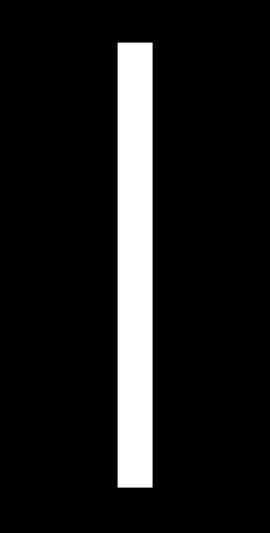
\includegraphics[width=1cm]{AB2-track2.png}
    \caption{Straight line to test the Alphabot2 RPi}
    \label{fig:fig8}
\end{figure}

\begin{figure}[H]
    \centering
    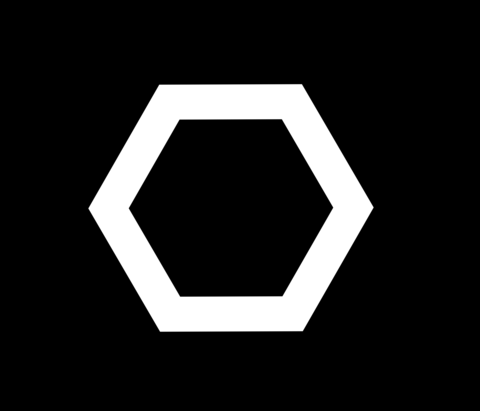
\includegraphics[width=3cm]{AB2-track3.png}
    \caption{Hexagonal track to test the Alphabot2 RPi}
    \label{fig:fig81}
\end{figure}


\subsection{Architecture} \label{ros}

Figure \ref{fig:fig9} represents the node architecture used, so that it is possible to interconnect the real and simulated Alphabot2 RPi, allowing its movement and the fulfillment of the objectives of this activity.

\begin{figure}[H]
    \centering
    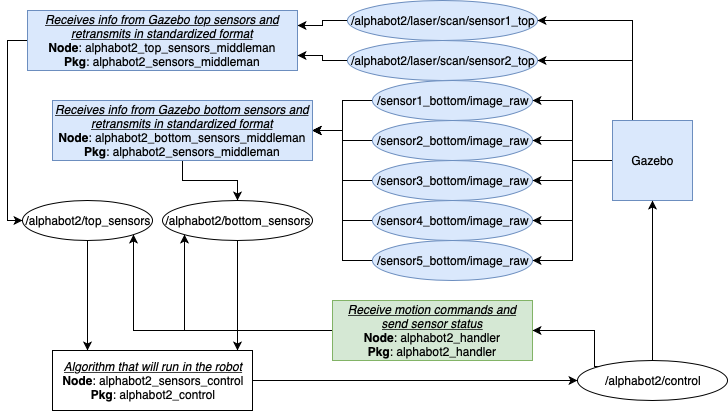
\includegraphics[width=9cm]{arch.png}
    \caption{Alphabot2 RPi architecture}
    \label{fig:fig9}
\end{figure}

This architecture can be summarized by the following steps:

\begin{enumerate}
    \item Upper and bottom sensors read their values and publish those values on their respective topics
    \item ``alphabot2\_top\_sensors\_middleman'' receives info from Gazebo top sensors and retransmits in standardized format to topic ``alphabot2/top\_sensors''
    \item ``alphabot2\_bottom\_sensors\_middleman'' receives info from Gazebo bottom sensors and retransmits in standardized format to topic ``alphabot2/bottom\_sensors''
    \item Then, an algorithm running on the package ``alphabot2\_control'' will execute the robot and its different behaviours
    \item Finally, the node ``/alphabot2\_handler'' through the node ``/alphabot2/contol'' receives motion commands and send sensor status to the middleman sensors topics (``alphabot2/top\_sensors'' and ``alphabot2/bottom\_sensors'')
\end{enumerate}

\subsection{Approach} \label{alg}

In order for the real and simulated Alphabot2 RPi to achieve the desired goals, it was necessary to create different algorithms that would allow them to avoid obstacles and to follow lines.

Most of the code used by the real robot was taken from the demo code on the Alphabot2 website, so one can program both its software and its hardware. Even so, it was still necessary to change some details, namely the linear and angular velocity translated values in the real Alphabot, so that both the real and the simulated robot walked at equal speeds when searching for the line to follow or avoid obstacles.

\subsubsection{Ros Topics} \label{topics}

Firstly, we defined the different ROS topics where the sensors would publish the values they scanned.

The two upper sensors, represented by laser scanners, which detect obstacles, publish their results for the following topics:

\begin{itemize}
    \item ``/alphabot2/laser/scan/sensor1\_top''
    \item ``/alphabot2/laser/scan/sensor2\_top''
\end{itemize}

The five bottom sensors, represented by camera sensors to detect the lines' brightness, publish their results for the following topics:

\begin{itemize}
    \item ``/sensor1\_bottom/image\_raw''
    \item ``/sensor2\_bottom/image\_raw''
    \item ``/sensor3\_bottom/image\_raw''
    \item ``/sensor4\_bottom/image\_raw''
    \item ``/sensor5\_bottom/image\_raw''
\end{itemize}

These results will be subscribed on the side of the algorithms to be evaluated and later published to other ROS topics, to be subscribed either by the real robot or by the simulated robot.

These new ROS topics will be described below.

\subsubsection{Obstacle Avoidance} \label{obs}

To detect obstacles, we first check whether the values read by the two upper sensors are infinite values. If these values were not infinite, it means that the sensors were able to detect an obstacle, by creating an array with two boolean values representing the detection of obstacles by each of the sensors, which would be published for the topic ``/alphabot2/top\_sensors'' (The approach explained can be found in Appendix \ref{appA}).

After this initial analysis, the robot subscribed to the topic ``/alphabot2/top\_sensors'' checks the values that were published there.

If it turns out that the left sensor has a value of true, it means that there was an obstacle on the left and therefore the robot would have to turn right (with a minimal linear velocity of 0.1m/s and an angular velocity of -0.6m/s$^{2}$). If it turns out that the right sensor is true, it means that there was an obstacle on the right and that the robot would have to turn left (with a minimal linear velocity of 0.1m/s and an angular velocity of 0.6m/s$^{2}$)(The code explained can be found in Appendix \ref{appC}).

\subsubsection{Line Following} \label{line}

To follow lines, we first calculate the brightness percentage scanned by the five bottom sensors, publishing them on the topic ``/alphabot2/bottom\_sensors''(The implementation explained can be found in Appendix \ref{appB}).

After this initial analysis, the robot subscribed to the topic ``/alphabot2/bottom\_sensors'' checks the brigthness values that were published there.

Initially, the minimum and maximum brightness captured by the robot and the deviation of brightness values for the lateral sensors and the central sensors were calculated. If the line has not yet been found and the maximum brightness is less than 50\%, the robot will search the line, with a linear velocity of 0.4m/s and an angular velocity of -0.1m/s$^{2}$. If that conditions did not occur some other conditions will be tested. If the brightness of middle sensor is greater than 50\% the line was found.
If the absolute difference between the brightness of the two intermediate sensors is less than 50 and either of these two has brightness above 50, the robot is on top of the line and will have to move forward with a linear velocity of 0.4m/s.
If the maximum brightness (among all sensors) is above 50 and the absolute difference between the brightness of the 2 edge sensors is less than 50, the robot will have to slightly correct its trajectory, having a linear velocity of 0.4m/s and an angular velocity of 0.1m/s$^{2}$ multiplied by a 1 or -1, depending on the turning direction.
%If the brightness value of the central sensor is greater than 50 and the maximum deviation value of the central sensors is less than 50, the robot will have to really correct its path, having a linear velocity of 0.1m/s and an angular velocity of 0.6m/s$^{2}$) multiplied by the inverse of the edge deviation value. 
%If the brightness value of the central sensor is greater than 50, the robot will have to correct its path very strongly, having a linear velocity of 0m/s and an angular velocity of 0.6m/s$^{2}$) multiplied by the inverse of the edge deviation value.
If none of the previously described cases occurs, the robot will have to completely change its trajectory, adopting a linear velocity of -0m/s and an angular velocity of 0.1m/s$^{2}$ multiplied by a 1 or -1, depending on the turning direction. (The code explained can be found in Appendix \ref{appC}).


\section{Results} \label{results}

In order to test the implemented implementation, so that the real and simulated robot could follow lines and avoid obstacles, some tests were done. The two robots were tested in two different lanes, one of 0.89m in a straight line and one of hexagonal shape with 0.30m of side, in order to test its movement and its execution time. In addition, the robots were also tested with obstacles to be avoided.

Thus, 6 different measurements were performed, for 3 different tests, each in its respective lane or with the robot that was related to it. The \textbf{T1} test represents the robots test in the straight line track, with no obstacle in the course. The \textbf{T2} test evaluates the robots in the straight line track with an obstacle in the course. The last one, the \textbf{T3} test, verifies the robots in the hexagonal track, with no obstacles in the main course. The measured times are shown in Table \ref{tab:tab1}.

\begin{table}[H]
\begin{center}
\begin{tabular}{ c c c }
\hline
  & Simulated Robot & Real Robot \\ 
 \hline
 T1 & 24s 68ms & 18s 02ms \\  
 T2 & 32s 62ms & 16s 53ms \\
 T3 & 2m 42s 35ms & 23s 73ms \\
 \hline
\end{tabular}
\caption{Time results captured.\label{tab:tab1}}\\
\end{center}
\end{table}

The absolute and relative errors of the measurements made were also calculated, according to the following formulas, respectively:

\[
    E_a_b_s = |x - x'|
\]

\[
    E_r_e_l = \frac{|x'- x|}{x}
\]

The results can be verified in Table \ref{tab:tab2}.

\begin{table}[H]
\begin{center}
\begin{tabular}{ c c c }
\hline
  & Absolute Error & Relative Error \\ 
 \hline
 T1 & 6,66 & 36,9589345\% \\  
 T2 & 16,09 & 97,338173\%  \\
 T3 & 138,62 & 584,155078\%  \\
 \hline
\end{tabular}
\caption{Absolute and relative errors.}
\label{tab:tab2}
\end{center}
\end{table}

\section{Conclusions} \label{conclusions}
Through the analysis of the obtained results, it is possible to conclude that this implementation allows the real Alphabot2 RPi and the simulated to follow lines and to avoid obstacles.

In addition, it was concluded that the real robot presents better values than the simulated robot, regardless of the track used for testing. This may be due to errors in either the Alphabot size measurements or the construction of the actual and simulated Gazebo tracks, as well as errors due to the positioning of the two robots in the different tracks. In addition, the fact that Alphabot2 is using some code already on the vendor's website may be causing it to perform better.

With all the results obtained, it is verified that the two robot implementation are not perfectly equal and their use together has some limitations. Even though in simpler tests such as T1 and T2 the performance was, tough very different, similar enough to demonstrate the concept works, in T3 we can see how much work still needs to be done.

As an interesting enhancement of the implemented work, we would like to create a way of synchronizing between the actual and the simulated Alphabot in order to be executed at the same time. A more practical enhancement would be to enhance the simulation model of the Alphabot, so that it would not oscillate so much when making turns and changing speeds.

\begin{thebibliography}{00}
\bibitem{b1} Costa, Valter, Peter Cebola, Armando Sousa, and Ana Reis. 2018. “Design Hints for Efficient Robotic Vision - Lessons Learned from a Robotic Platform.” Lecture Notes in Computational Vision and Biomechanics 27. Springer Netherlands: 515–24. doi:10.1007/978-3-319-68195-5\_56.
\bibitem{b2} Costa, Valter, Rosaldo Rossetti, and Armando Sousa. 2017. “Simulator for Teaching Robotics, ROS and Autonomous Driving in a Competitive Mindset.” International Journal of Technology and Human Interaction 13 (4): 19–32. doi:10.4018/IJTHI.2017100102.
\bibitem{b3} Bu, Yi, Binglu Wang, Win bin Huang, Shangkun Che, and Yong Huang. 2018. “Using the Appearance of Citations in Full Text on Author Co-Citation Analysis.” Scientometrics 116 (1). Springer Netherlands: 275–89. doi:10.1007/s11192-018-2757-z.
\bibitem{b4} Roy, Abhishek, and Mathew Mithra Noel. 2016. “Design of a High-Speed Line Following Robot That Smoothly Follows Tight Curves.” Computers and Electrical Engineering 56 (November). Elsevier Ltd: 732–47. doi:10.1016/j.compeleceng.2015.06.014.
\bibitem{b5} Matczak, Grzegorz, and Przemysław Mazurek. 2017. “Dim Line Tracking Using Deep Learning for Autonomous Line Following Robot.” In Advances in Intelligent Systems and Computing, 573:414–23. Springer Verlag. doi:10.1007/978-3-319-57261-1\_41.
\bibitem{b6} Javed, Mudassir, Sohail Hamid, Muhammad Talha, Zubair Ahmad, Fazle Wahab, and Hazrat Ali. 2018. “Input Based Multiple Destination, Multiple Lines Following Robot with Obstacle Bypassing.” ICST Transactions on Scalable Information Systems 5 (16): 154472. doi:10.4108/eai.13-4-2018.154472.
\bibitem{b7} Tanveer, M. Hassan, Carmine T. Recchiuto, and Antonio Sgorbissa. 2019. “Analysis of Path Following and Obstacle Avoidance for Multiple Wheeled Robots in a Shared Workspace.” Robotica 37 (1): 80–108. doi:10.1017/S0263574718000875.
\bibitem{b8} Matczak, Grzegorz, and Przemysław Mazurek. 2016. “Tracklet-Based Viterbi Track-Before-Detect Algorithm for Line Following Robots.” In , 649–58. doi:10.1007/978-3-319-26227-7\_61.
\bibitem{b9} 15th International Conference on Ubiquitous Robots, {UR} 2018, Honolulu, HI, USA, June 26-30, 2018. IEEE. 2018. Retrived from \url{http://ieeexplore.ieee.org/xpl/mostRecentIssue.jsp?punumber=8424588}. isbn:978-1-5386-6334-9.
\bibitem{b10} 3rd International Conference on Computing, Communication, Control and Automation (ICCUBEA-2017), August, 2017. IEEE. 2017. Retrived from \url{http://apps.webofknowledge.com/full_record.do?product=WOS&search_mode=GeneralSearch&qid=19&SID=E1Sb736VNEXNGjBndQd&page=5&doc=46&cacheurlFromRightClick=no}
\end{thebibliography}

\vspace{12pt}

\onecolumn
\appendix
\subsection{Appendix A} \label{appA}

\begin{lstlisting}[
    basicstyle=\tiny
]
import rospy
import message_filters
from std_msgs.msg import Int32MultiArray
from sensor_msgs.msg import LaserScan
from geometry_msgs.msg import Twist
import math

algorithmTopic = None

def callback(sensor1, sensor2):
    global algorithmTopic

    msg = Int32MultiArray()
    foundLeft = False
    foundRight = False

    for s in sensor1.ranges:
        if not math.isinf(s):
            foundRight = True

    for s in sensor2.ranges:
        if not math.isinf(s):
            foundLeft = True

    msg.data = [foundRight, foundLeft]


    algorithmTopic.publish(msg)


def main():
    global algorithmTopic

    rospy.init_node('alphabot2_top_sensors_middleman')

    algorithmTopic = rospy.Publisher('/alphabot2/top_sensors', Int32MultiArray, queue_size=1)

    sub1 = message_filters.Subscriber('/alphabot2/laser/scan/sensor1_top', LaserScan)
    sub2 = message_filters.Subscriber('/alphabot2/laser/scan/sensor2_top', LaserScan)

    ts = message_filters.TimeSynchronizer([sub1, sub2], 10)
    ts.registerCallback(callback)

    rospy.spin()

if __name__ == '__main__':
    main()
\end{lstlisting}

\subsection{Appendix B} \label{appB}

\begin{lstlisting}[
    basicstyle=\tiny
]
import rospy
import message_filters
from std_msgs.msg import Int32MultiArray
from sensor_msgs.msg import LaserScan, Image
from geometry_msgs.msg import Twist
from cv_bridge import CvBridge, CvBridgeError
import cv2
import numpy as np

algorithmTopic = None

def callback(sensor1, sensor2, sensor3, sensor4, sensor5):
  global algorithmTopic

  msg = Int32MultiArray()
  bridge = CvBridge()
  brightness1 = round(np.mean(cv2.cvtColor(bridge.imgmsg_to_cv2(sensor1, "bgr8"),cv2.COLOR_BGR2GRAY).flatten())*100/255)
  print(brightness1)

  brightness2 = round(np.mean(cv2.cvtColor(bridge.imgmsg_to_cv2(sensor2, "bgr8"),cv2.COLOR_BGR2GRAY).flatten())*100/255)
  print(brightness2)

  brightness3 = round(np.mean(cv2.cvtColor(bridge.imgmsg_to_cv2(sensor3, "bgr8"),cv2.COLOR_BGR2GRAY).flatten())*100/255)
  print(brightness3)

  brightness4 = round(np.mean(cv2.cvtColor(bridge.imgmsg_to_cv2(sensor4, "bgr8"),cv2.COLOR_BGR2GRAY).flatten())*100/255)
  print(brightness4)

  brightness5 = round(np.mean(cv2.cvtColor(bridge.imgmsg_to_cv2(sensor5, "bgr8"),cv2.COLOR_BGR2GRAY).flatten())*100/255)
  print(brightness5)

  msg.data = [brightness1, brightness2, brightness3, brightness4, brightness5]

  algorithmTopic.publish(msg)


def main():
  global algorithmTopic

  rospy.init_node('alphabot2_bottom_sensors_middleman')

  algorithmTopic = rospy.Publisher('/alphabot2/bottom_sensors', Int32MultiArray, queue_size=1)

  sub1 = message_filters.Subscriber('/sensor1_bottom/image_raw', Image)
  sub2 = message_filters.Subscriber('/sensor2_bottom/image_raw', Image)
  sub3 = message_filters.Subscriber('/sensor3_bottom/image_raw', Image)
  sub4 = message_filters.Subscriber('/sensor4_bottom/image_raw', Image)
  sub5 = message_filters.Subscriber('/sensor5_bottom/image_raw', Image)

  ts = message_filters.TimeSynchronizer([sub1, sub2, sub3, sub4, sub5], 10)
  ts.registerCallback(callback)

  rospy.spin()

if __name__ == '__main__':
  main()
\end{lstlisting}

\subsection{Appendix C} \label{appC}

\begin{lstlisting}[
    basicstyle=\tiny
]
import rospy
import message_filters
from std_msgs.msg import Int32MultiArray
from geometry_msgs.msg import Twist
from threading import Lock

HIGH_LINEAR_SPEED = 0.8
LOW_LINEAR_SPEED = 0.6

HIGH_ANGULAR_SPEED = 2.5
LOW_ANGULAR_SPEED = 1.5


movementTopic = None
bottomSensors = None
topSensors = None
lock = Lock()

lineNeverFound = True
prev_speed = 0
prev_z_sign = 0

def sign(x):
  if x < 0: return -1
  elif x > 0: return 1
  else: return 0

def calculateMovement(sensorsTop, sensorsBottom):
  global movementTopic
  global lineNeverFound
  global prev_speed
  global prev_z_sign

  msg = Twist()
  obstacleRight, obstacleLeft = sensorsTop.data
  print(sensorsTop.data)
  if obstacleLeft: 
    print "Obstacle found on the left. Turning right"
    msg.linear.x = LOW_LINEAR_SPEED
    msg.angular.z = - HIGH_ANGULAR_SPEED
  elif obstacleRight:
    print "Obstacle found on the right. Turning left"
    msg.linear.x = LOW_LINEAR_SPEED
    msg.angular.z = HIGH_ANGULAR_SPEED
  else:

    brightness1, brightness2, brightness3, brightness4, brightness5 = sensorsBottom.data
    print(sensorsBottom.data)
    #'''
    min_brightness = min(brightness1, brightness2, brightness3, brightness4, brightness5)
    max_brightness = max(brightness1, brightness2, brightness3, brightness4, brightness5)
    mid_deviation = brightness2 - brightness4  # >0 means more white on the right side. ranges from aprox [-100, 100]
    edge_deviation = brightness1 - brightness5 # >0 means more white on the right side
    str_turn = "right" if edge_deviation > 0 else "left"
    z_sign = -sign(edge_deviation)
    print("max: "+str(max_brightness)+", min: "+str(min_brightness)+", mid_dev: "+str(mid_deviation)+", edge_dev: "+str(edge_deviation))

    if lineNeverFound and max_brightness < 50:
      print("Looking for the line")
      msg.linear.x = HIGH_LINEAR_SPEED
      msg.angular.z = -0.1
    else:
      lineNeverFound = False
      if abs(mid_deviation) < 50 and max(brightness2, brightness4) > 50:
        print("Staying in the line")
        msg.linear.x = LOW_LINEAR_SPEED
        msg.angular.z = 0

      elif abs(edge_deviation) < 50 and max_brightness > 50: # little hope
        print("Warning! Correcting course to the "+str_turn)
        msg.linear.x = LOW_LINEAR_SPEED
        msg.angular.z = z_sign*HIGH_ANGULAR_SPEED
      else: # true panic
        print("PANICKING while correcting course!")
        z_sign = prev_z_sign
        msg.linear.x = - LOW_LINEAR_SPEED
        msg.angular.z = z_sign*LOW_ANGULAR_SPEED
    prev_z_sign = z_sign
  s1 = sign(prev_speed)
  s2 = sign(msg.linear.x)
  if s1*s2 < 0:
    msg.linear.x = prev_speed + msg.linear.x
  else:
    msg.linear.x = (prev_speed+msg.linear.x)/3
  prev_speed = msg.linear.x
  movementTopic.publish(msg)


def callbackTop(sensors):
  global topSensors
  global bottomSensors

  lock.acquire()
  if bottomSensors is not None:
    bottom = bottomSensors
    top = sensors
    bottomSensors = None
    topSensors = None
    lock.release()
    calculateMovement(top, bottom)
  else:
    lock.release()
    topSensors = sensors


def callbackBottom(sensors):
  global topSensors
  global bottomSensors

  lock.acquire()
  if topSensors is not None:
    bottom = sensors
    top = topSensors
    bottomSensors = None
    topSensors = None
    lock.release()
    calculateMovement(top, bottom)
  else:
    lock.release()
    bottomSensors = sensors


def main():
  global movementTopic

  rospy.init_node('alphabot2_sensors_control')

  movementTopic = rospy.Publisher('/alphabot2/control', Twist, queue_size=1)

  rospy.Subscriber('/alphabot2/top_sensors', Int32MultiArray, callbackTop)
  rospy.Subscriber('/alphabot2/bottom_sensors', Int32MultiArray, callbackBottom)

  rospy.spin()

if __name__ == '__main__':
  main()
\end{lstlisting}


\end{document}
